



\section{Wprowadzenie}
Celem tego rozdziału jest przedstawienie pracy projektowej aplikacji webowej wspomagającej naukę języków obcych za pomocą filmów i seriali. W kolejnych sekcjach opisano architekturę systemu, projekt bazy danych, implementację logiki aplikacji oraz jej frontendu i backendu, zabezpieczenia przed redundancją danych oraz niepoprawnymi wpisami, możliwość logowania z różnych urządzeń obsługujących przeglądarki, implementację różnych metod nauki oraz elementów gamifikacji.
\section{Przypadki użycia}

\section{Baza danych}

\subsection{Wprowadzenie}
Do przechowywania danych aplikacji wykorzystano bazę danych NoSQL MongoDB Atlas. Baza danych składa się z kilku kolekcji, które przechowują informacje o użytkownikach, napisach, słowach. Wszystkie kolekcje są połączone relacjami, które umożliwiają szybkie wyszukiwanie i filtrowanie danych.

MongoDB Atlas to usługa bazodanowa w chmurze oferowana przez firmę MongoDB. Jest to w pełni zarządzana platforma, która umożliwia łatwe tworzenie, zarządzanie i skalowanie baz danych MongoDB. Atlas oferuje wiele funkcji, takich jak automatyczne tworzenie kopii zapasowych, monitorowanie wydajności, automatyczne skalowanie, a także wysoki poziom bezpieczeństwa dzięki szyfrowaniu danych w spoczynku i w tranzycie.

Jedną z głównych zalet MongoDB Atlas jest jego elastyczność i skalowalność. Użytkownicy mogą łatwo dostosować zasoby bazy danych do swoich potrzeb, zwiększając lub zmniejszając moc obliczeniową oraz przestrzeń dyskową w zależności od wymagań aplikacji. Atlas obsługuje również replikację danych, co zapewnia wysoką dostępność i odporność na awarie.

MongoDB Atlas integruje się z wieloma popularnymi platformami chmurowymi, takimi jak AWS, Google Cloud Platform i Microsoft Azure, co pozwala na łatwe wdrożenie bazy danych w preferowanym środowisku chmurowym. Dodatkowo, Atlas oferuje narzędzia do analizy danych, takie jak MongoDB Charts, które umożliwiają tworzenie interaktywnych wizualizacji danych bezpośrednio z bazy danych. 


\subsection{Struktura}
W kontekście aplikacji, MongoDB Atlas zapewnia niezawodne i skalowalne rozwiązanie do przechowywania danych użytkowników, sesji użytkownika, napisów, słów oraz zdań, co umożliwia szybkie i efektywne wyszukiwanie oraz filtrowanie informacji. Dane są przechowywane w kolekcjach, które zawierają dokumenty w formacie JSON (JavaScript Object Notation). Każda kolekcja może zawierać dokumenty o różnej strukturze, co zapewnia dużą elastyczność w przechowywaniu danych.

Aby przyspieszyć wyszukiwanie danych, MongoDB umożliwia tworzenie indeksów na polach dokumentów. Indeksy mogą znacznie poprawić wydajność zapytań, zwłaszcza w przypadku dużych zbiorów danych. W aplikacji wykorzystano indeksy domyślnie na relacjach i kluczach obcych, aby zapewnić szybkie wyszukiwanie i filtrowanie danych.
MongoDB jest bazą danych schemaless, co oznacza, że dokumenty w tej samej kolekcji mogą mieć różne struktury. Dzięki temu możemy łatwo dostosowywać strukturę danych do zmieniających się wymagań aplikacji.

Dodatkowo, MongoDB zapewnia wysoką dostępność i skalowalność poprzez replikację i sharding. Replikacja polega na utrzymywaniu wielu kopii danych na różnych serwerach, co zwiększa niezawodność i dostępność bazy danych. Sharding pozwala na podział danych na mniejsze fragmenty, które są przechowywane na różnych serwerach, co umożliwia skalowanie poziome bazy danych.

Poniżej przedstawiono diagram struktury bazy danych, który ilustruje relacje między poszczególnymi kolekcjami.
\begin{figure}[H]
    \centering
    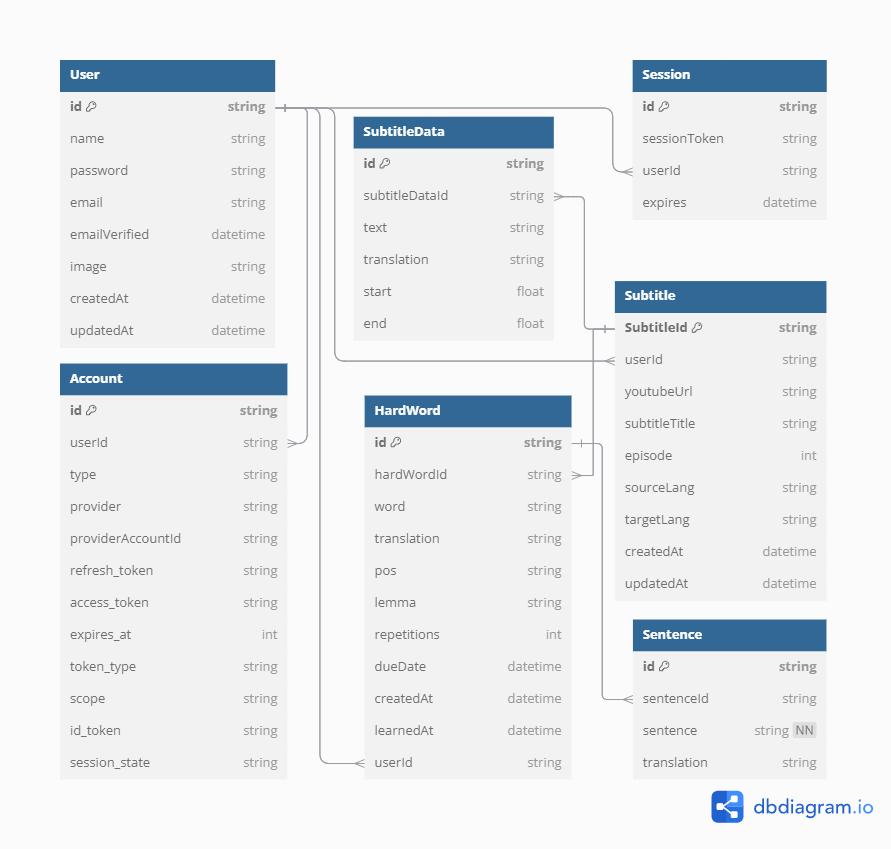
\includegraphics[width=1\textwidth]{IMAGE/DatabaseDiagram.png}
    \caption{Diagram struktury bazy danych}
    \label{fig:StrukturaBazyDanych}
\end{figure}
\subsection{Metody zapobiegania redundancji danych}
W celu zapobiegania redundancji danych w aplikacji zastosowano kilka metod. Przede wszystkim, projekt bazy danych został starannie zaplanowany, aby zminimalizować duplikację danych. Wykorzystano normalizację danych, która polega na podziale danych na mniejsze, logicznie powiązane tabele lub kolekcje, co pozwala na uniknięcie powtarzania tych samych informacji w różnych miejscach.

Dodatkowo, w aplikacji zaimplementowano mechanizmy walidacji danych, które sprawdzają poprawność i spójność danych przed ich zapisaniem do bazy. Dzięki temu możliwe jest wykrycie i eliminacja ewentualnych duplikatów na etapie wprowadzania danych. Poza jednym duplikatem, którym jest kolekcja zdania "sentence" gdy użytkownik usunie napisy z kolekcji "subtitles" to wtedy w kolekcji "sentence" pozostanie zdanie, które w trakcie nauki z słowami pozostaną bezpiecznie w bazie.

Wykorzystano również indeksy unikalne, które zapewniają, że w danej kolekcji nie mogą istnieć dwa dokumenty z identycznymi wartościami w polach, które powinny być unikalne. Na przykład, w kolekcji użytkowników zastosowano indeks unikalny na polu adresu e-mail, co zapobiega rejestracji dwóch użytkowników z tym samym adresem e-mail. W kolekcji słów zastosowano indeks unikalny na polu słowa "word", co zapobiega dodaniu dwóch  identycznych słów przez jednego użytkownika. To samo dotyczy kolekcji napisów, gdzie zastosowano indeks unikalny na polu tytułowym "subtitleTitle" w połączeniu z odcinkiem "episode" co nie pozwala przypadkowo dodać dwa takie same tytuły w połączeniu z odcinkiem.

Kolejną metodą zapobiegania redundancji jest stosowanie referencji między kolekcjami. Zamiast przechowywać duplikaty danych, dokumenty w jednej kolekcji mogą zawierać referencje do dokumentów w innych kolekcjach. Na przykład, dokumenty w kolekcji sesji użytkownika mogą zawierać referencje do dokumentów w kolekcji użytkowników, co pozwala na przechowywanie informacji o użytkownikach w jednym miejscu i uniknięcie redundancji.

Wszystkie te metody razem zapewniają, że dane w bazie są przechowywane w sposób efektywny i bez zbędnej redundancji, co przekłada się na lepszą wydajność i spójność danych.

\section{Interfejs użytkownika}
Interfejs użytkownika aplikacji składa się z kilku głównych widoków, które umożliwiają użytkownikom korzystanie z różnych funkcji. Wszystkie widoki zostały zaprojektowane z myślą o prostocie i intuicyjności, aby zapewnić użytkownikom łatwą nawigację i szybki dostęp do potrzebnych informacji. Poniżej przedstawiono najważniejsze elementy interfejsu użytkownika.


\subsection{Widok startowy}

\begin{figure}[H]
    \centering
    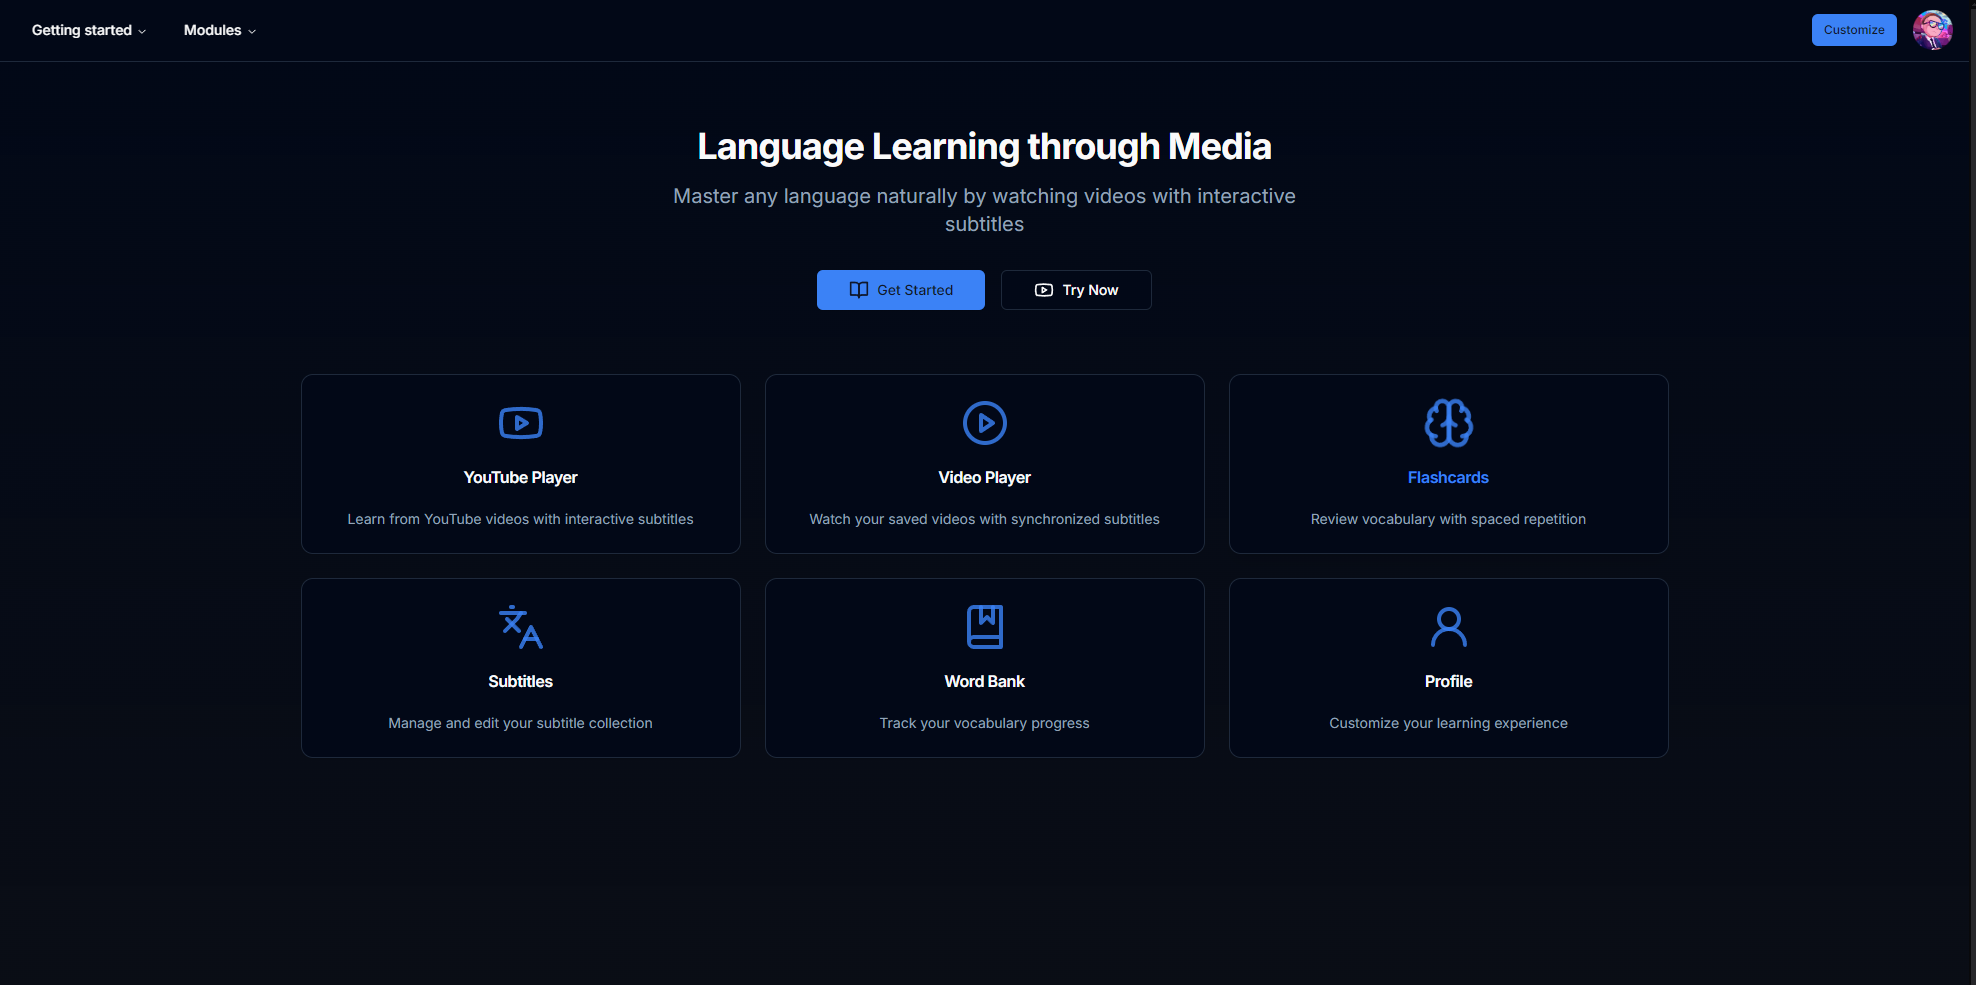
\includegraphics[width=1\textwidth]{IMAGE/HomePage.png}
    \caption{Strona główna aplikacji}
    \label{fig:Widok strony głównej aplikacji}
\end{figure}
Strona główna aplikacji zawiera przyciski kierujace do innych sekcji aplikacji, takich jak nauka, słownik, statystyki, profil użytkownika, ustawienia, itp. Użytkownicy mogą również przeglądać najnowsze filmy i seriale dostępne w aplikacji oraz korzystać z wyszukiwarki, aby znaleźć interesujące ich treści.

\subsection{Strona Nauki}

\begin{figure}[H]
    \centering
    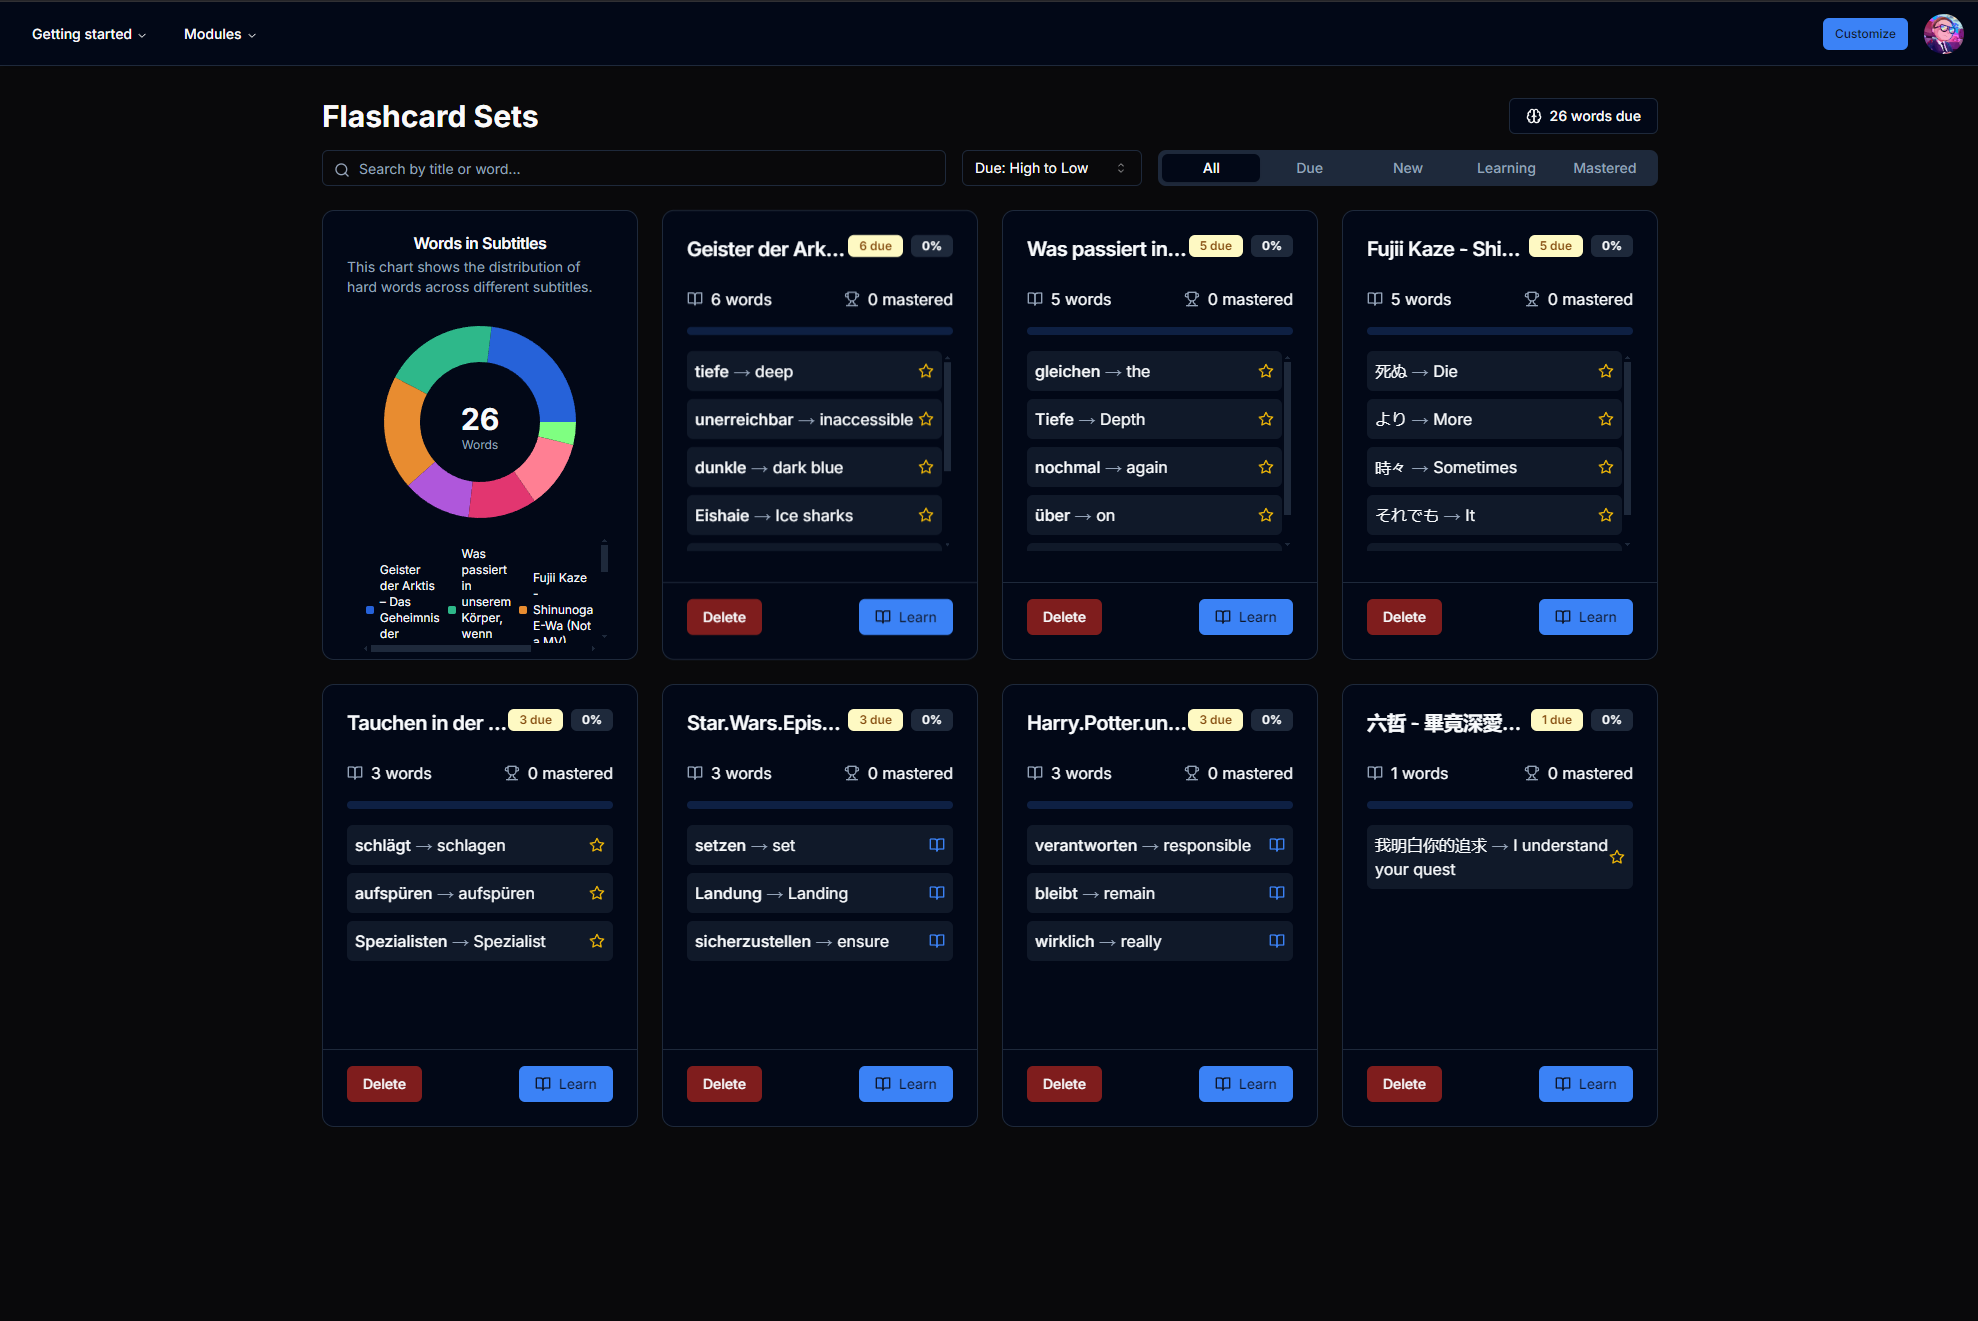
\includegraphics[width=1\textwidth]{IMAGE/FlashCards.png}
    \caption{Widok strony głównej fiszek}
    \label{fig:Strona głowna fiszek}
\end{figure}
\begin{figure}[H]
    \centering
    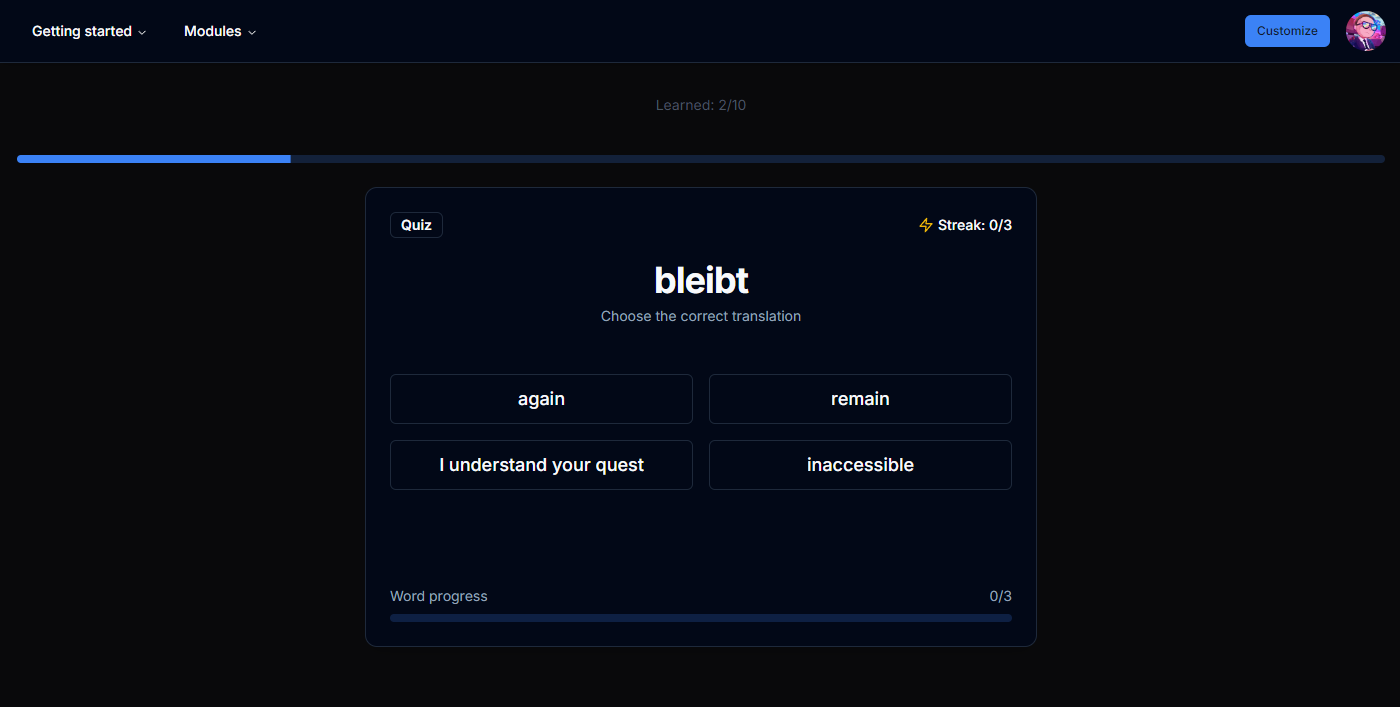
\includegraphics[width=1\textwidth]{IMAGE/Quiz.png}
    \caption{Widok quizu}
    \label{fig:Nauka z quizem}
\end{figure}
Strona Nauki to główne miejsce, w którym użytkownicy mogą korzystać z panelu nauki fiszek lub quizu. Panel fiszek zawiera informacje na temat stanu słów które są nowe, w trakcie nauki, lub skończone. Strona quizu umożliwia użytkownikom nauke poprzez quizy, w których użytkownicy muszą wybrać poprawne tłumaczenie słowa. Użytkownicy muszą poprawnie odpowiedzieć 3 razy z rzędu by słowo zostało uznane za nauczone i przeszło do kolejnego etapu którym jest powtórka po upływie odpowiedniego czasu.

\subsection{Strona Napisów}

\begin{figure}[H]
    \centering
    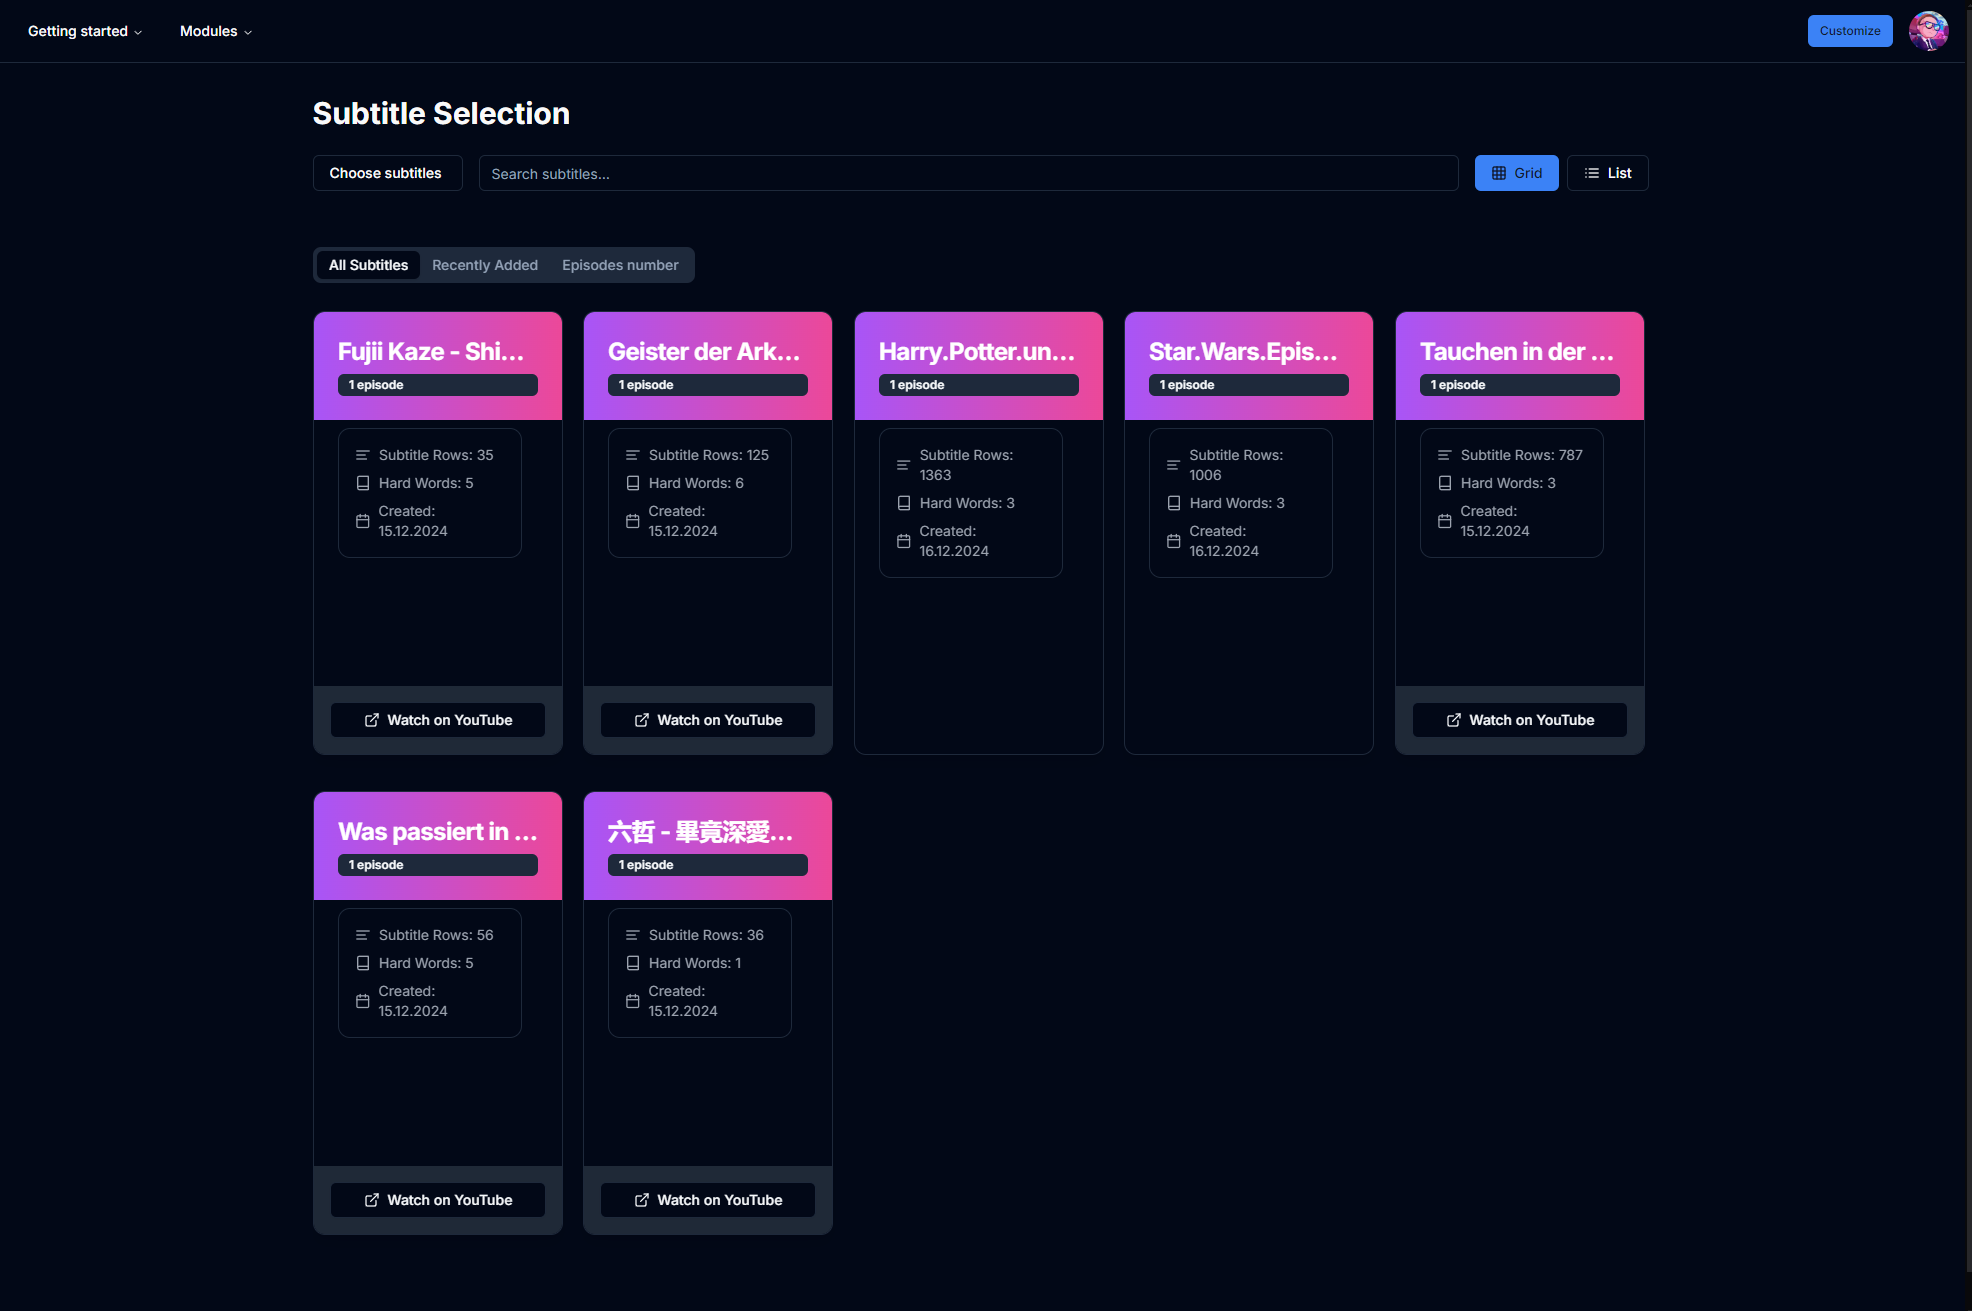
\includegraphics[width=1\textwidth]{IMAGE/Subtitles.png}
    \caption{Widok strony napisów}
    \label{fig:Strona napisów}
\end{figure}
Strona główna umożliwia wyszukiwanie zapisanych napisów, dostępne jest wyszukiwanie po tytule. Użytkownicy mogą również sortować napisy według daty dodania oraz liczby odcinków. Panel daje również możliwość zmiany wyświetlania między siatką a listą domyślnie jest to siatka maksymalnie 5 elementów na wiersz w zależności od miejsca na ekranie.

\begin{figure}[H]
    \centering
    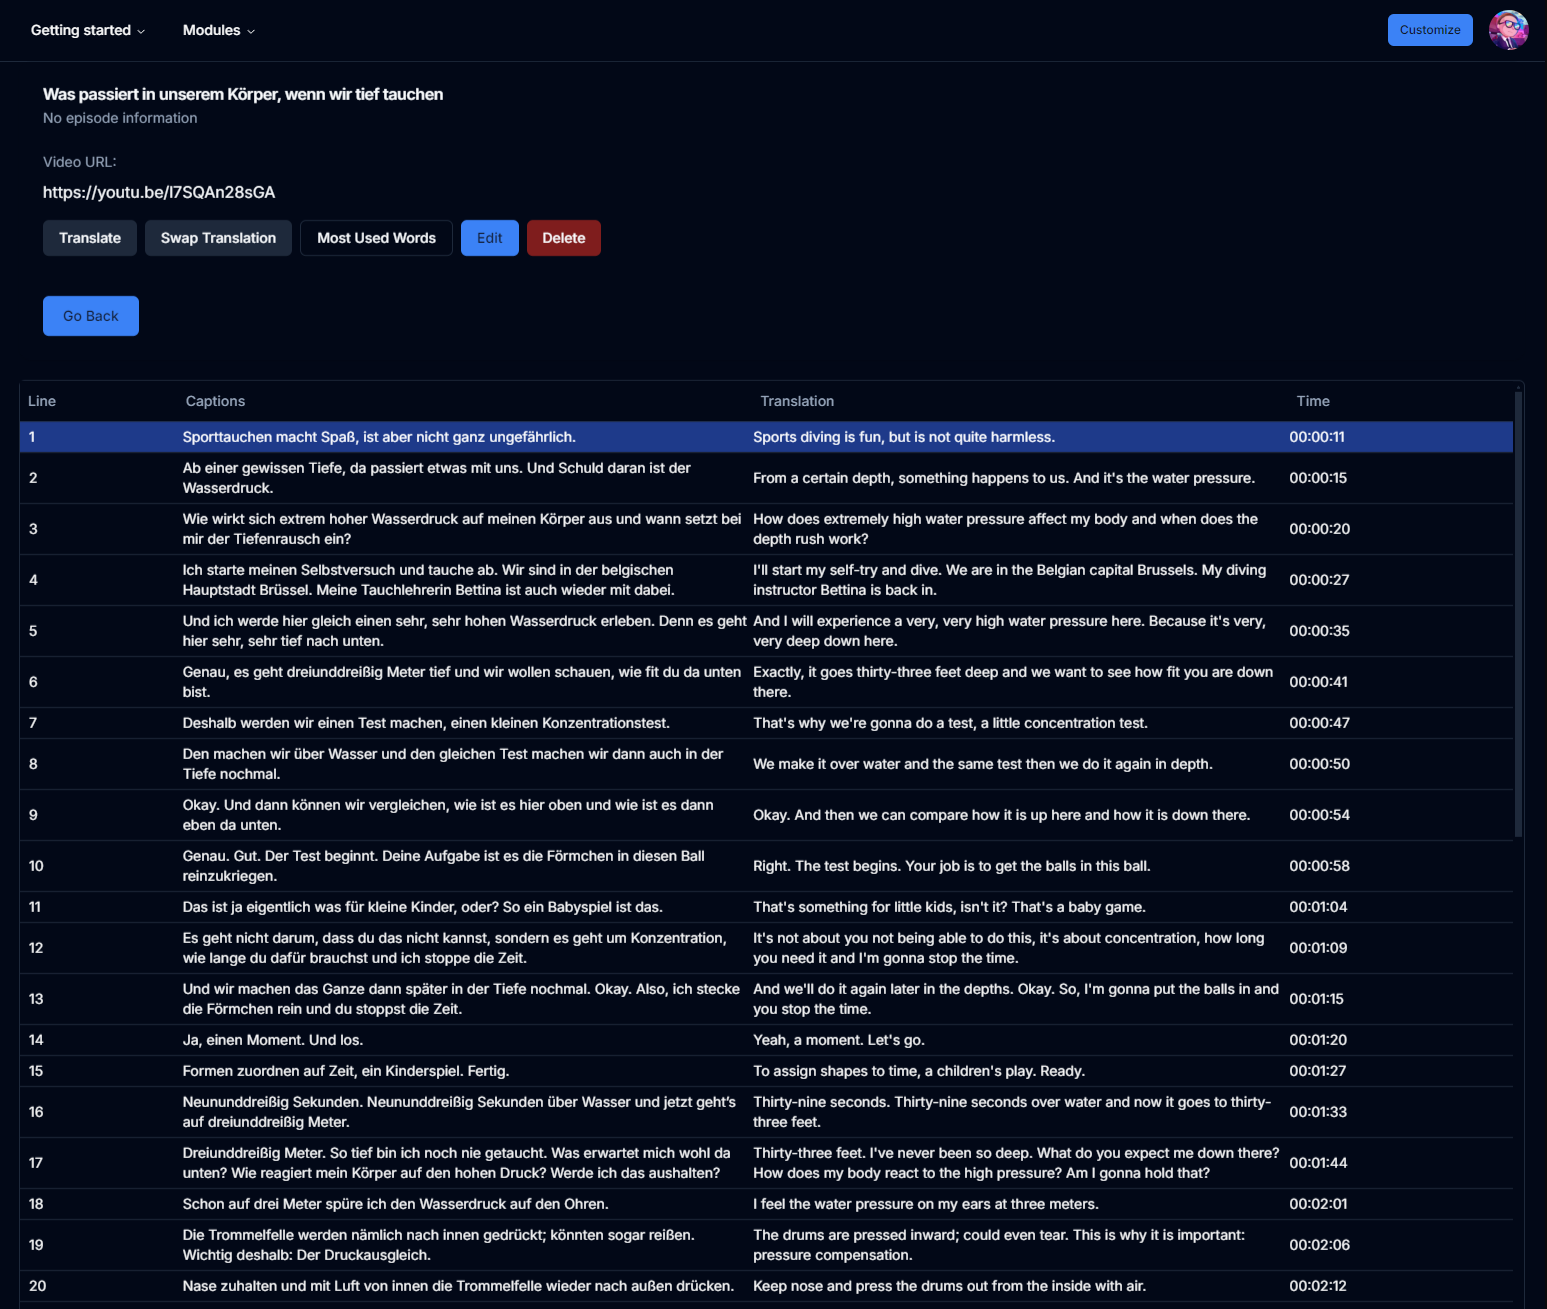
\includegraphics[width=1\textwidth]{IMAGE/SubtitlesSelected.png}
    \caption{Widok edycji napisów}
    \label{fig:Edycja napisów}
\end{figure}
Strona Napisów umożliwia użytkownikom przeglądanie i edycję napisów w bazie danych. Użytkownicy mogą edytować istniejące napisy, usuwać napisy, a także przeglądać listę wszystkich napisów w bazie z pomocą sortowania i wyszukiwania.

\subsection{Strona Słownika}

\begin{figure}[H]
    \centering
    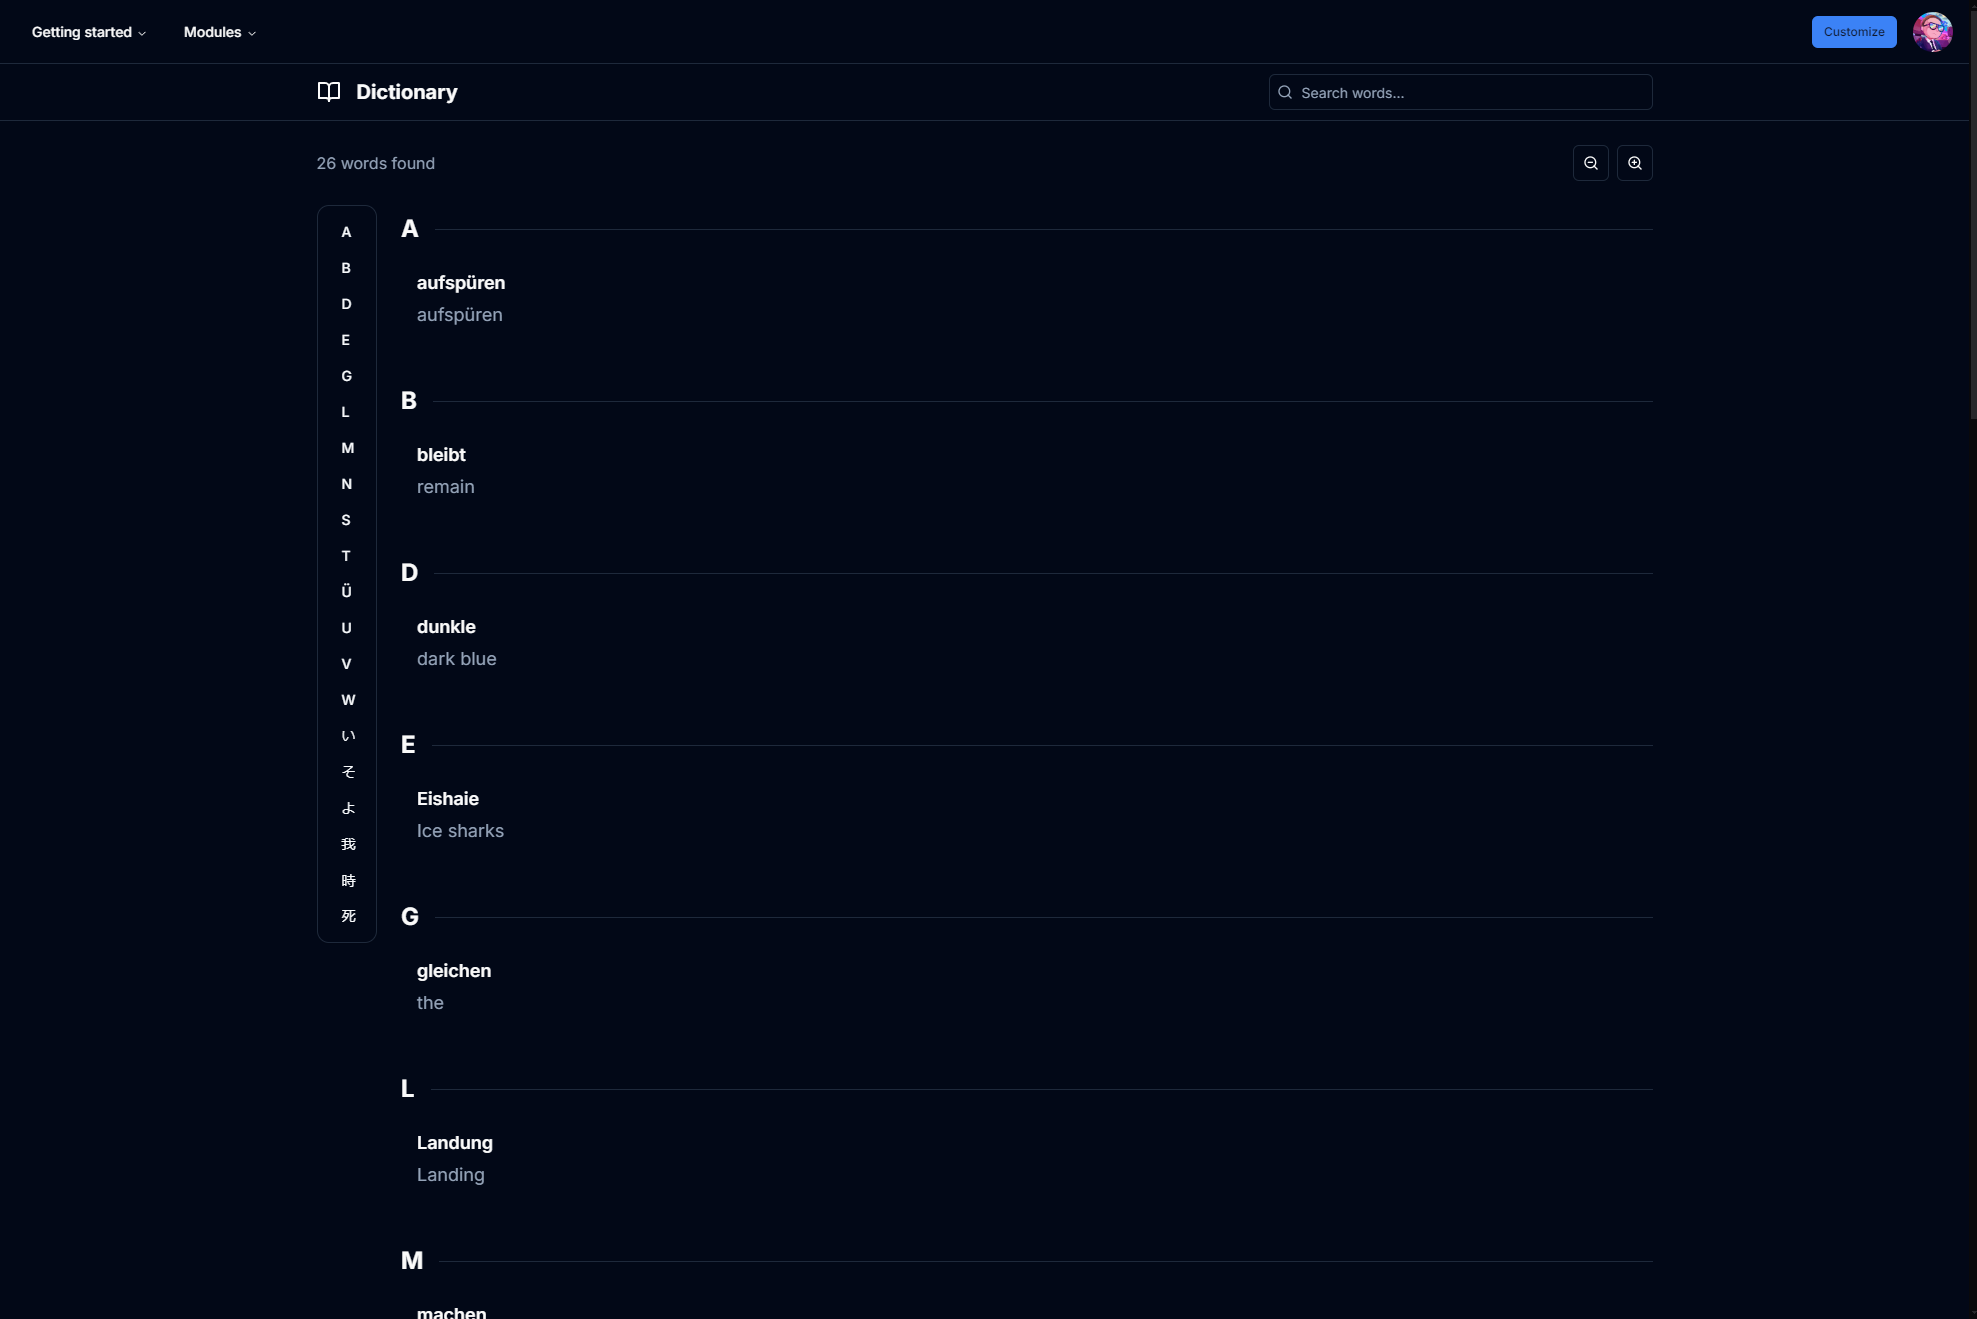
\includegraphics[width=1\textwidth]{IMAGE/WordBank.png}
    \caption{Widok słownika}
    \label{fig:Słownik słów}
\end{figure}
Strona Słownika umożliwia użytkownikom przeglądanie i edycję słów w bazie danych. Użytkownicy mogą  edytować istniejące słowa, usuwać słowa, a także przeglądać listę wszystkich słów w bazie z pomocą sortowania i wyszukiwania. Panel obsługuje również chińskie znaki.
\subsection{Strona Statystyk}

\begin{figure}[H]
    \centering
    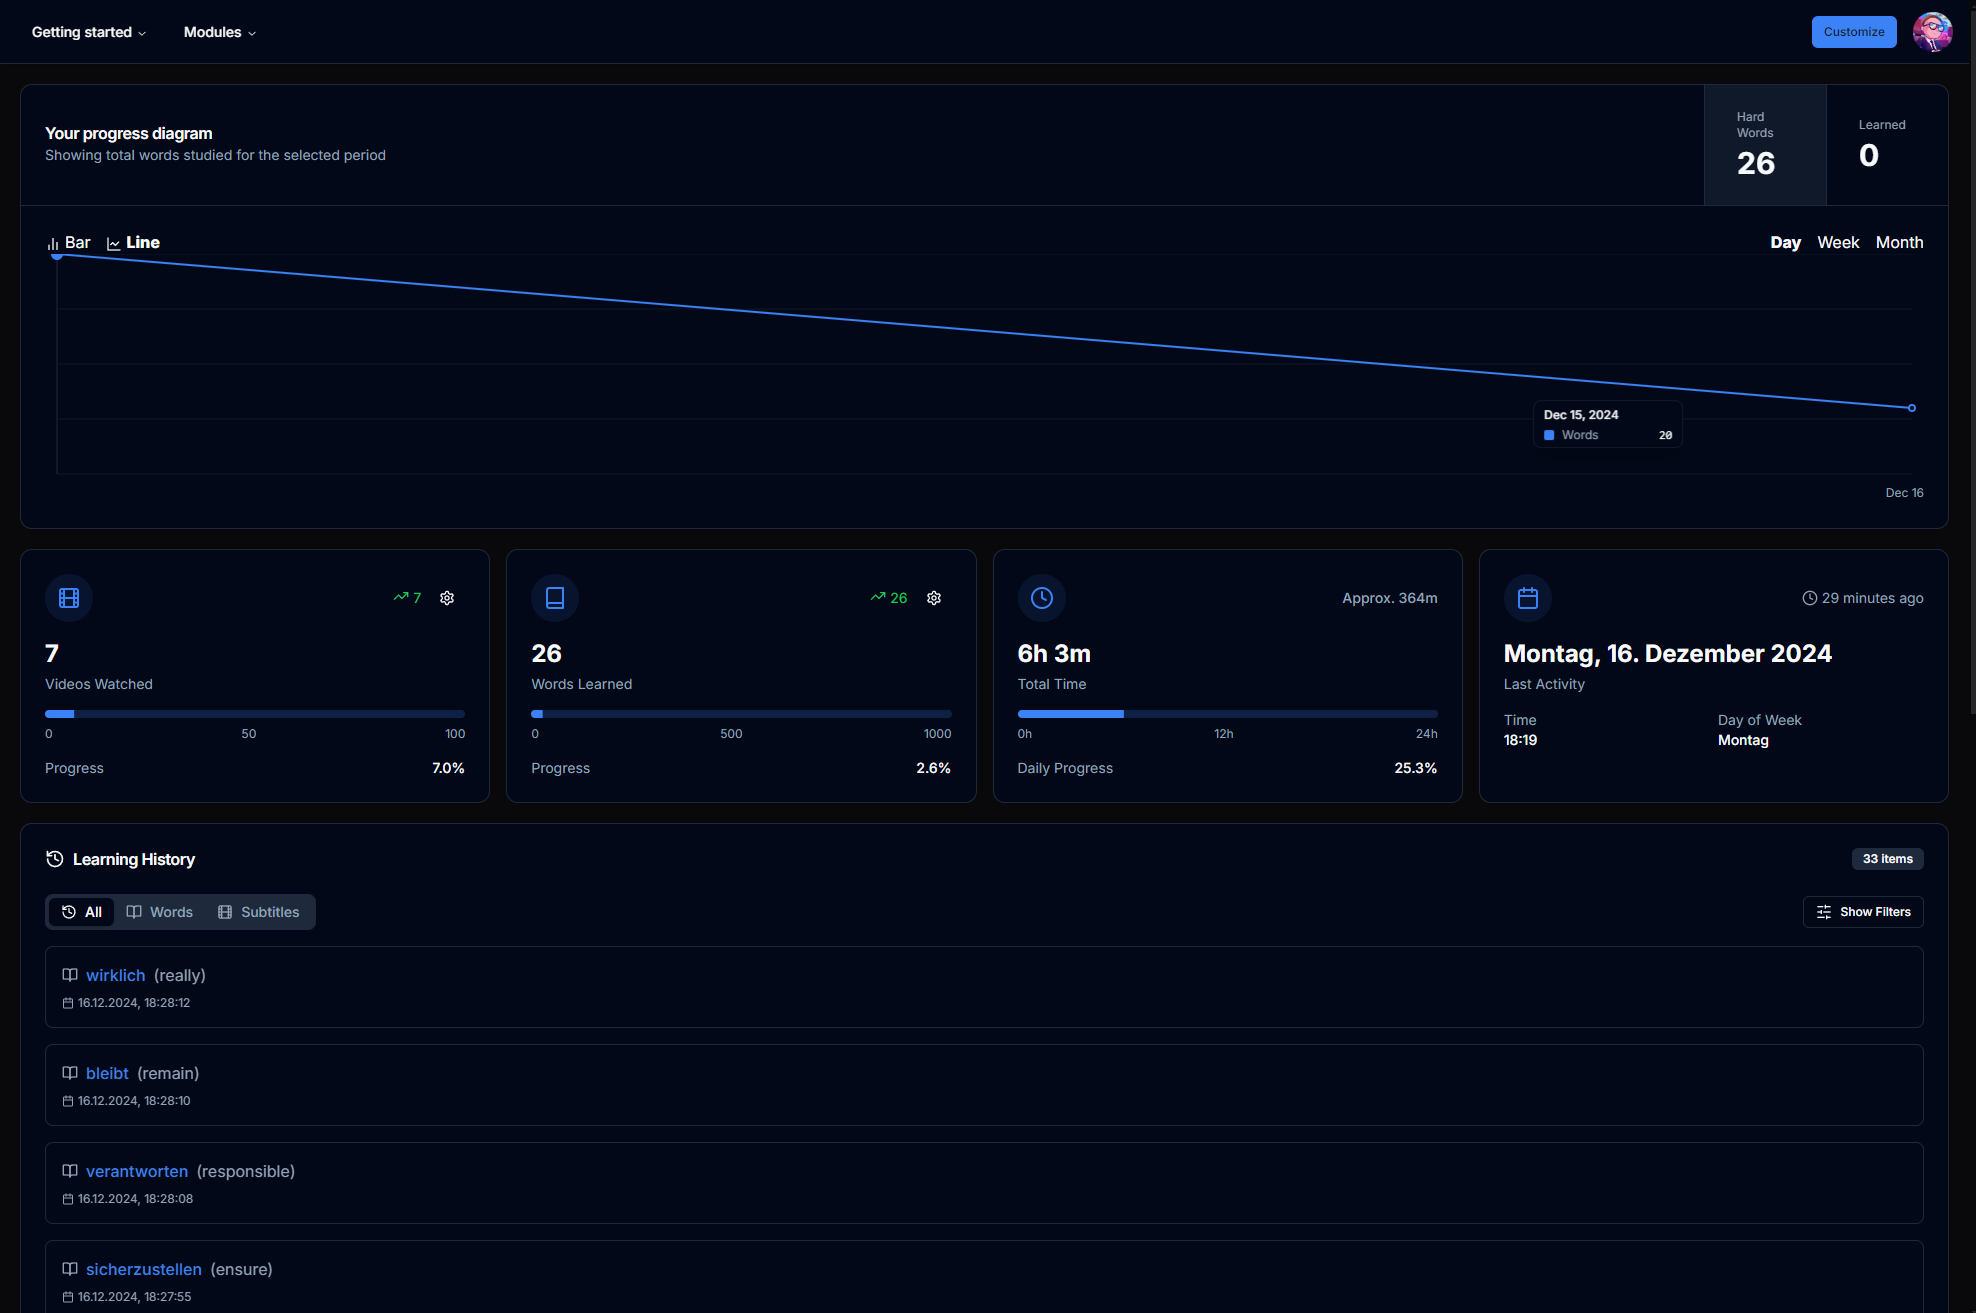
\includegraphics[width=1\textwidth]{IMAGE/Progress.png}
    \caption{Widok statystyk i postępów}
    \label{fig:Statystyki postępów}
\end{figure}
Strona Statystyk zawiera wykresy i statystyki dotyczące postępów w nauce użytkowników. Użytkownicy mogą śledzić swoje postępy w nauce słówek. Panel zawiera również informacje na temat liczby nowych słówek, oraz słówek nauczonych już wraz z datami utworzenia słowa i ukończenia nauki.
\subsection{Strona logowania oraz rejestracji}

\begin{figure}[H]
    \centering
    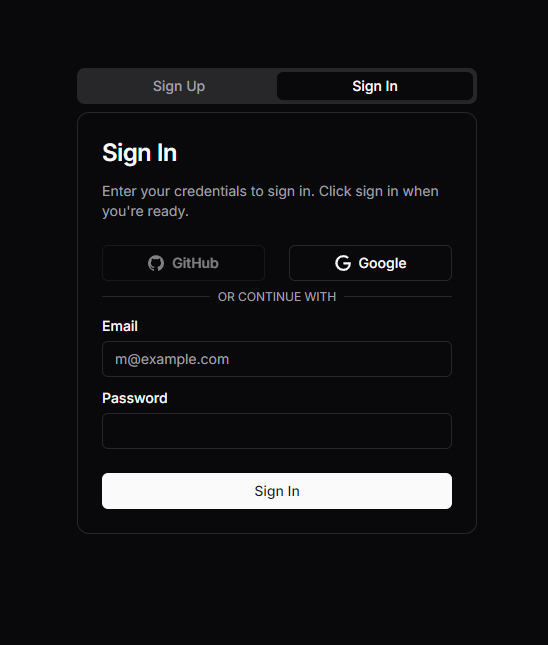
\includegraphics[width=1\textwidth]{IMAGE/LoginPage.png}
    \caption{Widok logowania i rejestracji}
    \label{fig:Logowanie i rejestracja}
\end{figure}
Strona logowania i rejestracji umożliwia użytkownikom zalogowanie się do aplikacji lub utworzenie nowego konta. Użytkownicy mogą wprowadzić swoje dane logowania, takie jak adres e-mail i hasło, aby uzyskać dostęp do aplikacji. Panel obsługuje również logowanie za pomocą konta Google, Logowanie za pomocą GitHub będzie dodane również pózniej.
\subsection{Strona oglądania filmów}


\begin{figure}[H]
    \centering
    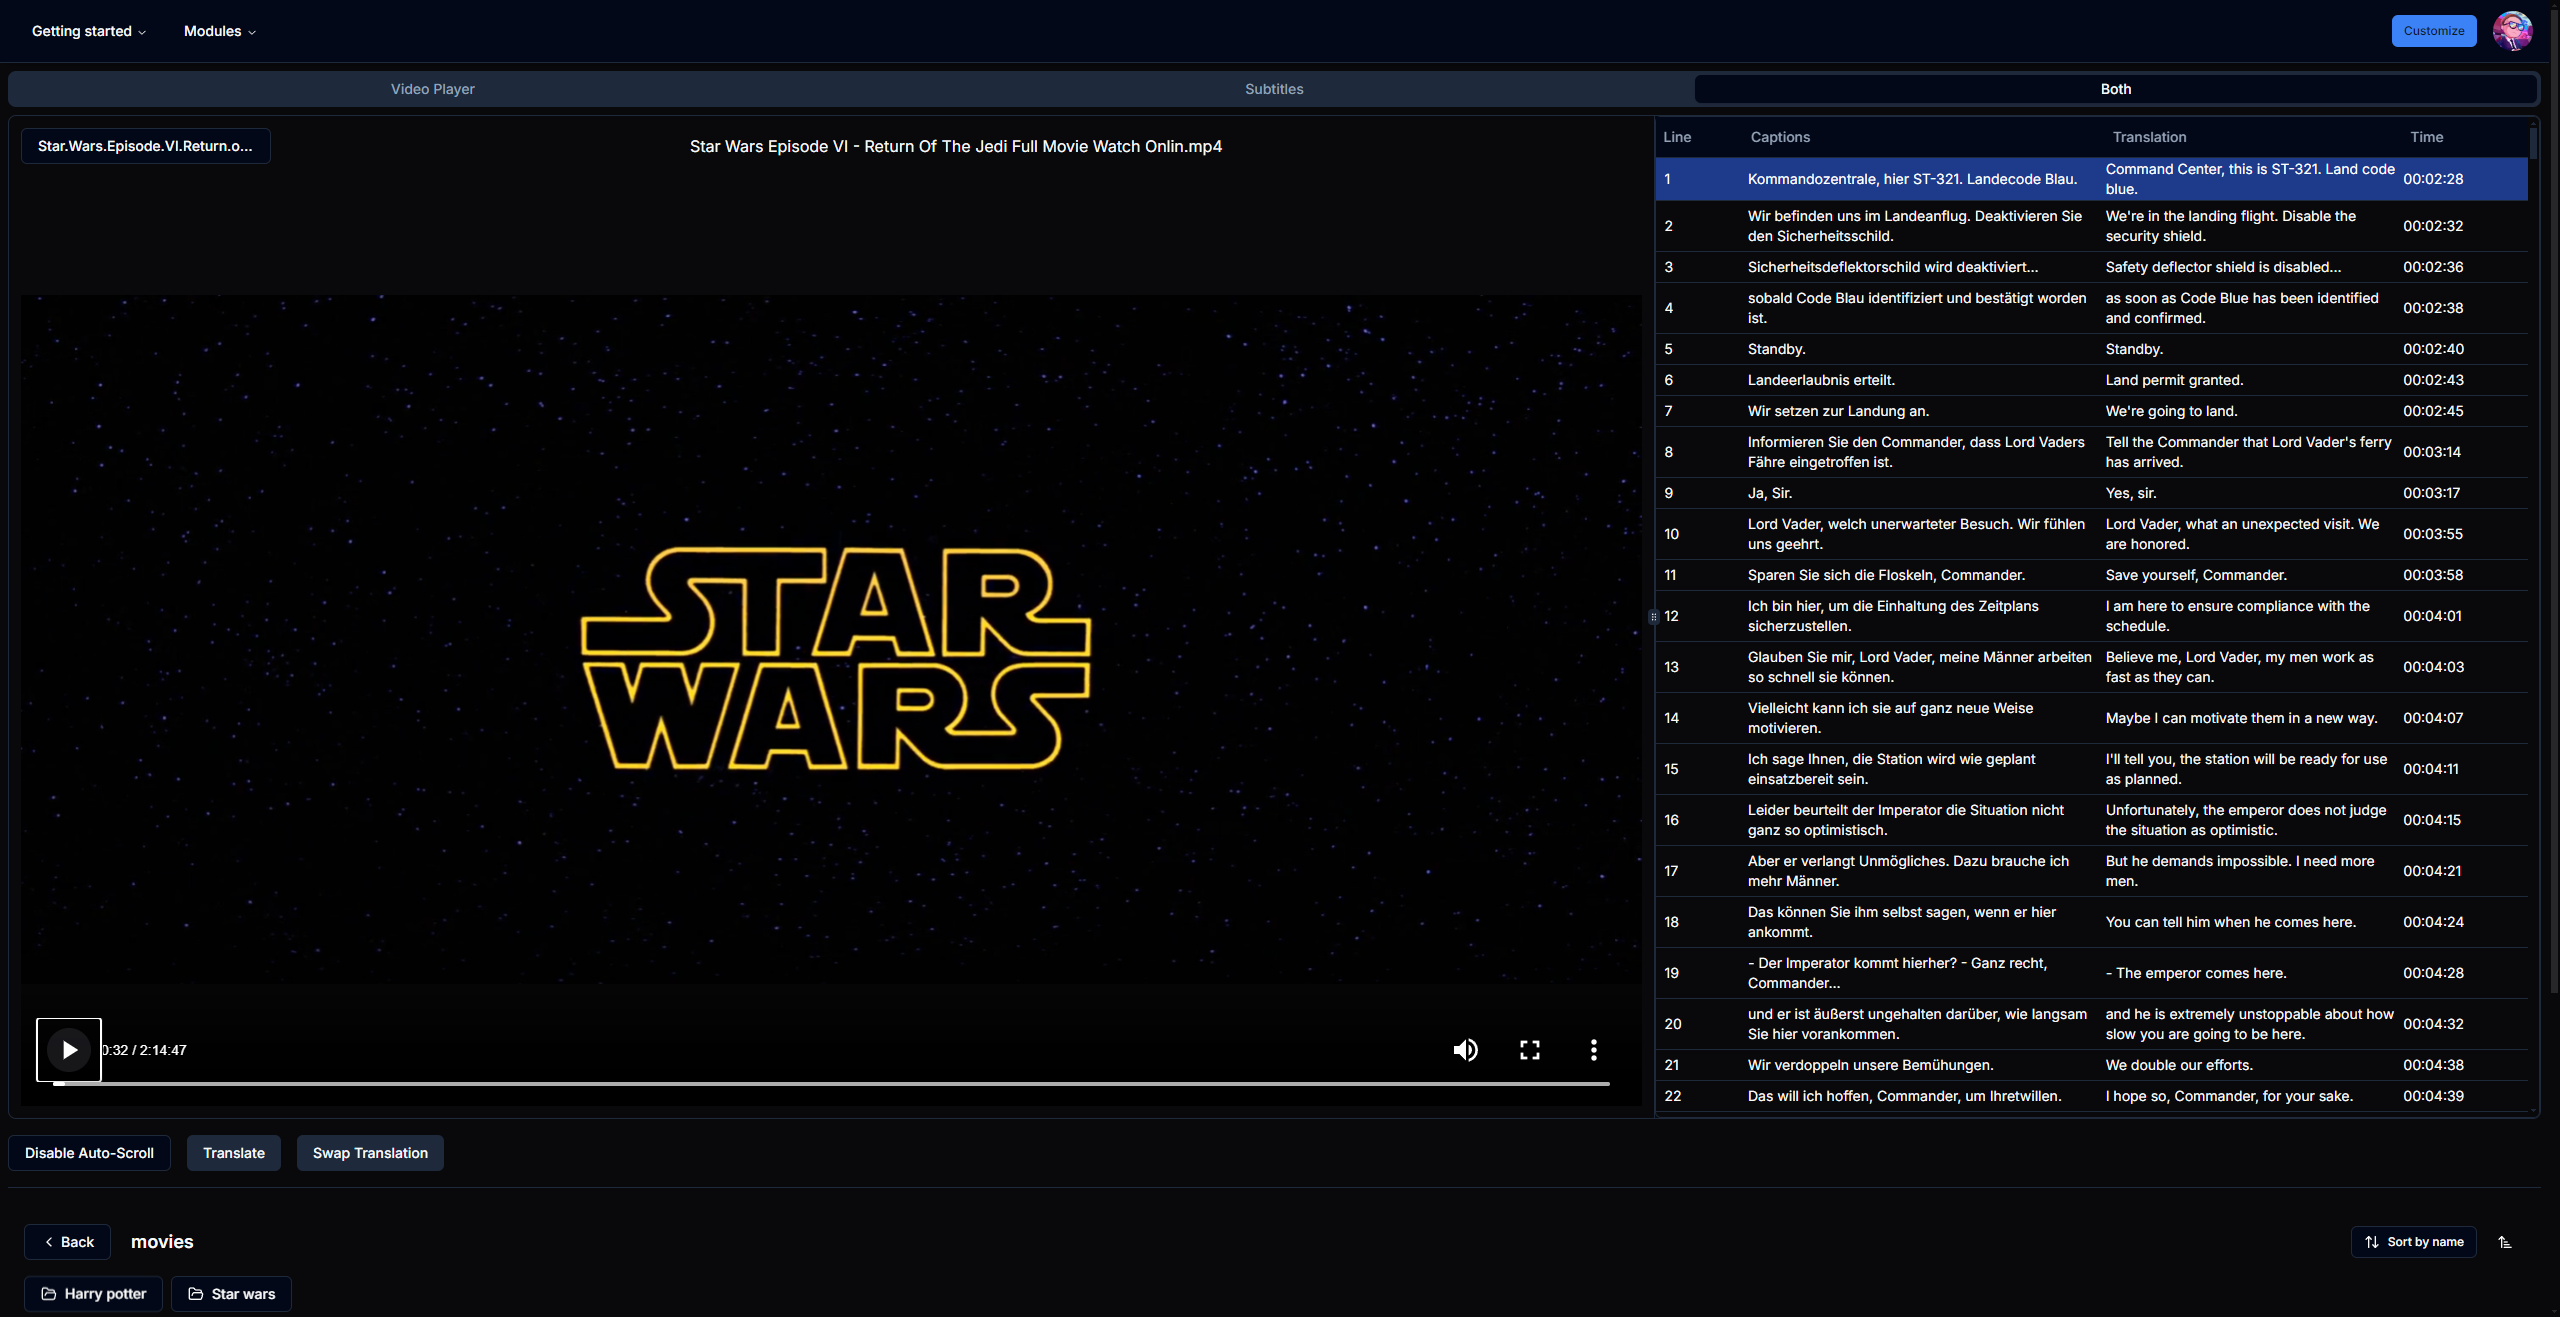
\includegraphics[width=1\textwidth]{IMAGE/videoPlayer.png}
    \caption{Widok oglądania filmów}
    \label{fig:oglądanie filmów}
\end{figure}

Strona oglądania filmów umożliwia użytkownikom przeglądanie i odtwarzanie filmów i seriali z listy zapisanych napisów i wybrania odpowiedniego filmu z dysku. Użytkownicy mogą zamienić szybko jezyk orginalny z przetłumaczonym lub włączyć śledzenie aktualnego wiersza napisów względem filmu "auto-scroll", a następnie rozpocząć oglądanie. Panel obsługuje również przewijanie filmu, zmianę języka napisów, oraz dodawanie słów do bazy w celu pózniejszej nauki. Użytkownik ma do wyboru albo filmy z rozszerzeniem mp4 albo mkv a napisy w formacie srt lub ass.




\section{Podsumowanie}
